\documentclass[a4paper,12pt]{scrartcl}
\usepackage[utf8]{inputenc}
\usepackage[UKenglish]{isodate}
\usepackage{csquotes}
\usepackage{graphicx}
\usepackage{wrapfig}
\usepackage{enumitem}
\usepackage{pdflscape}
\usepackage[toc,page]{appendix}
\usepackage{geometry}
\usepackage{hyperref}
\usepackage{cleveref}
\usepackage{listings}
\usepackage{csvsimple}
\usepackage{booktabs}
\usepackage{longtable}
\usepackage{caption}
\usepackage{subcaption}
\usepackage[colorinlistoftodos]{todonotes}
\usepackage[british]{babel}
\usepackage{float}
%\usepackage[margin=1in]{geometry}
\usepackage{listings}
\usepackage{color}
 
\definecolor{codegreen}{rgb}{0,0.6,0}
\definecolor{codegray}{rgb}{0.5,0.5,0.5}
\definecolor{codepurple}{rgb}{0.58,0,0.82}
\definecolor{backcolour}{rgb}{0.95,0.95,0.92}
 
\lstdefinestyle{mystyle}{
	language=PHP,
    backgroundcolor=\color{backcolour},   
    commentstyle=\color{codegray},
    keywordstyle=\color{magenta},
    numberstyle=\tiny\color{codegray},
    stringstyle=\color{codegreen},
    basicstyle=\footnotesize,
    breakatwhitespace=false,         
    breaklines=true,                 
    captionpos=b,                    
    keepspaces=true,                 
    numbers=left,                    
    numbersep=5pt,                  
    showspaces=false,                
    showstringspaces=false,
    showtabs=false,                  
    tabsize=3,
    morekeywords={ new, __halt_compiler, abstract, and, array, as, break, callable, case, catch, class, clone, const, continue, declare, default, die, do, echo, else, elseif, empty, enddeclare, endfor, endforeach, endif, endswitch, endwhile, eval, exit, extends, final, for, foreach, function, global, goto, if, implements, include, include_once, instanceof, insteadof, interface, isset, list, namespace, new, or, print, private, protected, public, require, require_once, return, static, switch, throw, trait, try, unset, use, var, while, xor}
}

\lstset{language=Java,
  showspaces=false,
  showtabs=false,
  breaklines=true,
  showstringspaces=false,
  breakatwhitespace=true,
  commentstyle=\color{pgreen},
  keywordstyle=\color{pblue},
  stringstyle=\color{pred},
  basicstyle=\ttfamily,
  moredelim=[il][\textcolor{pgrey}]{$$},
  moredelim=[is][\textcolor{pgrey}]{\%\%}{\%\%}
}
 
\lstset{style=mystyle}

\graphicspath{ {images/} }
\usepackage[
	backend=biber,
	style=ieee,
	]{biblatex}

\addbibresource{references.bib}

\title{829H1 Real-Time Embedded Systems Exercise 1}
\author{Candidate No: 105936}
\date{\today}

\begin{document}
	
	\begin{titlepage}
		\maketitle
	\end{titlepage}
	
	\tableofcontents
	\newpage
	
	\section{Introduction}
	{
		This report outlines the work completed during the laboratory sessions, what equipment was used and what was learnt. Code listings for some of the created programs can be found in \cref{Appendix:start}.
	}

	\section{Equipment}
	{
		\subsection{Hardware}{
			The experiments carried out in this report were run on the Freedom-K64F prototyping board\cite{nxpproducts2014}. To use this board, we needed to connect the board to the computer using the debug port and copy across the program we wish to run and then press the reset button to load the program.
			\begin{figure}[h]
				\centering
				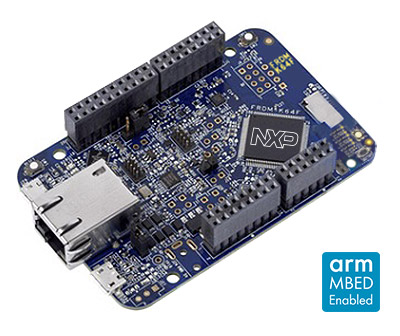
\includegraphics[width=0.5\textwidth]{FRDM-K64F-ANGLE}
				\caption{An Image of the Freedom-K64F Board used during experimentation\cite{nxpproducts2014}}
				\label{img:FRDM-K64F}
			\end{figure}
		}
		\subsection{Software}
		{
			To develop the experiments, I used Arm's mbed cloud IDE. This allows users to write c++ code and compile it to a device of their choice. 
		}
	}
	
	\section{Experiments}
	{
		\subsection{Interrupts}
		{
			Interrupts seem to work in a similar way to event handlers in other programming languages in that they allow you to run a function out of sequence which can be called from another object. In the example, the red led is being turned on and off when the button SW2 is being released this is because the function \lstinline|ISR1()| is being called when the button is released.
			\subsubsection{Interrupt triggered by falling edge}
			{
				This means that the code should be changed so that the function is called when the button is pressed not when its released therefore all we need to change is the \lstinline|button.rise(&ISR1);| to \lstinline|button.fall(&ISR1);| The code for this can be found in \cref{appendix:ex1-1}
			}
			\subsubsection{Two Interrupts on a single switch}
			{
				The interrupts I created worked by switching the green led when it was pressed down and the red led when released. This meant I had to create another function \lstinline|ISR2()| which would switch the green led. The code for this can be found in \cref{appendix:ex1-2}
			}
			
			\subsubsection{Showing the function runs independently of the while loop}
			{
				The led is being turned on and off independently of the while loop this can be shown by increasing the wait time in the loop so that the led can be turned on and off without the led flashing. The code for this can be found in \cref{appendix:ex1-3}
			}
		}
		\subsection{Timers}
		{
			This experiment makes use of the timers. Allowing programmers to time things in their programs.
			\subsubsection{Differing times for differing string lengths}
			{
				For this experiment, I created a program which would create strings of increasing length while timing how long it would take to output them to the terminal. The code for this can be found in \cref{appendix:ex2-1}.
				\begin{table}[]
					\centering
					\begin{tabular}{|c|c|c|c|}
						\hline
						\textbf{\begin{tabular}[c]{@{}c@{}}Character\\ Length\end{tabular}} & \textbf{String} & \textbf{\begin{tabular}[c]{@{}c@{}}Time taken to\\ print to screen\end{tabular}} & \textbf{\begin{tabular}[c]{@{}c@{}}Difference to one\\ fewer character length\end{tabular}} \\ \hline
						0 &  & 0.000019 &  \\ \hline
						1 & a & 0.002075 & 0.002056 \\ \hline
						2 & aa & 0.003114 & 0.001039 \\ \hline
						3 & aaa & 0.004154 & 0.00104 \\ \hline
						4 & aaaa & 0.005194 & 0.00104 \\ \hline
						5 & aaaaa & 0.006235 & 0.001041 \\ \hline
						6 & aaaaaa & 0.007275 & 0.00104 \\ \hline
						7 & aaaaaaa & 0.008314 & 0.001039 \\ \hline
						8 & aaaaaaaa & 0.009355 & 0.001041 \\ \hline
						9 & aaaaaaaaa & 0.010395 & 0.00104 \\ \hline
						10 & aaaaaaaaaa & 0.011435 & 0.00104 \\ \hline
					\end{tabular}
				\caption{Showing the time taken to print a string to the screen compared to the character length.}
				\label{tbl:TimeToPrintToScreen}
				\end{table} 
				\cref{tbl:TimeToPrintToScreen} shows that adding a character to the string after it is at least 1 character long takes around 0.00104 seconds.
			}
			\subsubsection{Using multiple timers}
			{
				Unfortunately, I did not have an oscilloscope to hand when running this experiment, therefore, looking at it by eye and as a slow-motion video. I can see that the red led(ledA) flashes every 0.2 seconds and the green led(ledB) flashes every second. 
			}
			\subsubsection{Using different repetition rates}
			{
				For this, I rewrote the task which turned the led on and off to work on the led passed to it meaning I only needed one method for all the leds. Although I still needed a timer for each led, therefore, had to initialise them at the start of the main function. The times I set were 0.2,0.3,0.4 and, 0.5 this lead to a flashy program as the led is changing colour every 0.1 seconds. The code for this can be found in \cref{appendix:ex2-2}
			}
		}
	}

	\section{Conclusion}
	{
		In conclusion, this was a useful quick introduction into how to develop using interrupts and timers also learning how to use tera term to view the console output of the board.
	}
	
	\newpage
	\begin{appendices}
	\label{Appendix:start}
	\section{Lab Exercise 1}
	{
		\subsection{Part 1}
		{
			\label{appendix:ex1-1}
			\lstinputlisting[language=c++]{CodeListings/Ex1/mainPart1.cpp}
		}
		\subsection{Part 2}
		{
			\label{appendix:ex1-2}
			\lstinputlisting[language=c++]{CodeListings/Ex1/mainPart2.cpp}
		}
		\subsection{Part 3}
		{
			\label{appendix:ex1-3}
			\lstinputlisting[language=c++]{CodeListings/Ex1/mainPart3.cpp}
		}
	}
	\section{Lab Exercise 2}
	{
		\label{appendix:ex2}
		\subsection{Part 1 - Master Program}
		{
			\label{appendix:ex2-1}
			\lstinputlisting[language=c++]{CodeListings/Ex2/main-master.cpp}
		}
		\subsection{Part 2 - Slave Program}
		{
			\label{appendix:ex2-2}
			\lstinputlisting[language=c++]{CodeListings/Ex2/main-slave.cpp}
		}
	}

\end{appendices}
	\printbibliography[heading=bibintoc,title=References]
\end{document}
